\section{PHƯƠNG TRÌNH BẬC HAI MỘT ẨN} % Tên bài
\subsection{Giải bài toán bằng cách lập phương trình bậc hai}
\begin{tomtat}
	Các bước để giải bài toán bằng cách lập phương trình bậc hai
	\begin{itemize}
		\item \text{Bước 1.} Lập phương trình
		\begin{itemize}
			\item Chọn ẩn và đặt điều kiện thích hợp cho ẩn.
			\item Biểu diễn các đại lượng chưa biết theo ẩn và các đại lượng đã biết.
			\item Lập phương trình biểu thị mối quan hệ giữa các đại lượng.
		\end{itemize}
		\item \text{Bước 2.} Giải phương trình nói trên.
		\item \text{Bước 3.}  Kiểm tra các nghiệm tìm được ở bước 2 có thoả mãn điều kiện của ẩn hay không, rồi trả lời bài toán.
	\end{itemize}
\end{tomtat}

\subsubsection{Bài toán thành lập số tự nhiên}
\begin{vd}%[9D4H2-5]%[GVSB: Nguyễn Văn Nghĩa-GVPB1:Hoàng Minh Nhân Mã-GVPB2: Phan Tấn Phú]
	 Cho một số tự nhiên có hai chữ số. Tổng hai chữ số của chúng bằng $10$. Tích hai chữ số ấy nhỏ hơn số đã cho là $12$. Tìm số đã cho.
	\loigiai{
	Gọi $x$ là chữ số hàng chục ($x\in\left\lbrace 1;2;3;\ldots;9\right\rbrace$).\\
	Do chữ số hàng chục và chữ số hàng đơn vị có tổng là $10$ nên ta có chữ số hàng đớn vị là $\left(10-x\right)$.\\
	Ta có giá trị của số đó là $10x+\left(10-x\right)$.\\
	Vì giá trị của số đó lớn hơn tích hai chữ số là $12$ nên ta có phương trình 
	\begin{eqnarray*}
		x\cdot\left(10-x\right)&= & 10x+10-x-12\\
		10x-x^2&= & 9x-2\\
		x^2-x-2&= & 0\\
		x = 2 \textrm{ (nhận) }   &\textrm{ hoặc }& x=-1 \textrm{ (loại).}
	\end{eqnarray*}
	Vậy số đã cho là $28$.
	}
\end{vd} 
%Bài 1
\begin{bt}%[9D4H2-5]%[GVSB: Nguyễn Văn Nghĩa-GVPB1:Hoàng Minh Nhân Mã-GVPB2: Phan Tấn Phú]
	 Tích của hai số tự nhiên liên tiếp lớn hơn tổng của chúng là $109$. Tìm hai số đó.
	\loigiai{
		Gọi $x$ là số thứ nhất ($x\in\mathbb{N^*}$).\\
		Số thứ hai là $\left(x+1\right)$.\\
		Tích hai số đó là $x\left(x+1\right)$.\\
		Tổng hai số đó là $x+\left(x+1\right)=2x+1$.\\
		Vì tích hai số đó lớn hơn tổng $109$ nên ta có phương trình 
		\begin{eqnarray*}
			x\cdot\left(x+1\right)&= & 2x+1+109\\
			x^2+x&= & 2x+110\\
			x^2-x-110&= & 0\\
			x = 11 \textrm{ (nhận) }   &\textrm{ hoặc }& x=-10 \textrm{ (loại).}
		\end{eqnarray*}
		Vậy hai số đã cho là $11$, $12$.
	}
\end{bt}
%Bài 2
\begin{bt}%[9D4H2-5]%[GVSB: Nguyễn Văn Nghĩa-GVPB1:Hoàng Minh Nhân Mã-GVPB2: Phan Tấn Phú]
	 Cho ba số tự nhiên liên tiếp. Tích của số đầu và số thứ ba lớn hơn ba lần số thứ hai là $549$. Tìm ba số tự nhiên đó.
\loigiai{
	Gọi $x$ là số thứ nhất ($x\in\mathbb{N^*}$).\\
	Số thứ hai là $\left(x+1\right)$.\\
	Số thứ ba là $\left(x+2\right)$.\\
	Vì tích của số đầu và số thứ ba lớn hơn $3$ lần số thứ hai là $549$ nên ta có phương trình
	\begin{eqnarray*}
		x\cdot\left(x+2\right)-3\cdot\left(x+1\right)&= & 549\\
		x^2+2x-3x-3&= & 549\\
		x^2-x-552&= & 0\\
		x = 24 \textrm{ (nhận) }   &\textrm{ hoặc }& x=-23 \textrm{ (loại).}
	\end{eqnarray*}
	Vậy ba số đã cho là $24$, $25$, $26$.
}
 \end{bt}
 \begin{bt}%[9D4V2-5]%[GVSB: Nguyễn Văn Nghĩa-GVPB1:Hoàng Minh Nhân Mã-GVPB2: Phan Tấn Phú]
 	 Tìm số tự nhiên có hai chữ số biết rằng $2$ lần chữ số hàng chục lớn hơn chữ số hàng đơn vị là $7$ đơn vị và $3$ lần chữ số hàng chục lớn hơn tích của hai chữ số là $8$.
 \loigiai{
 Gọi $x$ là chữ số hàng chục ($x\in\left\lbrace 1;2;3;\ldots;9\right\rbrace$).\\
 Vì $2$ lần chữ số hàng chục lớn hơn chữ số hàng đơn vị là $7$ nên chữ số hàng đơn vị là $2x-7$, ($x>3$).\\
 Vì $3$ lần chữ số hàng chục lớn hơn tích của hai chữ số là $8$, ta có phương trình 
 	\begin{eqnarray*}
 	3x-x\cdot\left(2x-7\right)&= & 8\\
 	3x-2x^2+7x&= & 8\\
 	-2x^2+10x-8&= & 0\\
 	x = 4 \textrm{ (nhận) }  &\textrm{ hoặc }&x= 1 \textrm{ (loại).}
 \end{eqnarray*}
 Vậy số đã cho là $41$.
 }
 \end{bt} 
 
 \subsubsection{Bài toán chuyển động}
 
 \begin{vd}%[9D4H2-5]%[GVSB: Nguyễn Văn Nghĩa-GVPB1:Hoàng Minh Nhân Mã-GVPB2: Phan Tấn Phú]
 	Khoảng cách giữa hai thành phố Hà Nội và Hạ Long là khoảng $156$ km. Ô tô thứ nhất khởi hành từ Hà Nội đến Hạ Long với vận tốc không đổi. Sau đó $24$ phút, ô tô thứ hai cùng khởi hành từ Hà Nội đến Hạ Long (trên cùng tuyến đường với ô tô thứ nhất) với vận tốc lớn hơn vận tốc của ô tô thứ nhất là $8$ km/h. Biết rằng cả hai ô tô đều đến Hạ Long cùng một lúc. Tính vận tốc của mỗi ô tô.
 	\loigiai{
 		Đổi $24$ phút $=\dfrac{24}{60}=\dfrac{2}{5}$ giờ.\\
 		Gọi $x$ (km/h) là vận tốc của ô tô thứ nhất $(x>0)$.\\
 		Khi đó, vận tốc của ô tô thứ hai là $x+8$ (km/h).\\
 		Khoảng cách giữa hai thành phố là $156$ km nên
 		\begin{itemize}
 			\item Thời gian đi của ô tô thứ nhất là $\dfrac{156}{x}$ (giờ).
 			\item Thời gian đi của ô tô thứ hai là $\dfrac{156}{x+8}$ (giờ).
 		\end{itemize}
 		Theo đề bài, ô tô thứ hai khởi hành sau ô tô thứ nhất $\dfrac{2}{5}$ giờ và cả hai ô tô đều đến Hạ Long cùng một lúc, nên ta có phương trình
 		\allowdisplaybreaks
 		\begin{eqnarray*}
 			\dfrac{156}{x} &=& \dfrac{156}{x+8}+\dfrac{2}{5}\\
 			780(x+8) &=& 780x + 2x(x+8) \\
 			x^2+8x-3\,120 &=& 0.
 		\end{eqnarray*}
 		Giải phương trình, ta được $x = 52$ (nhận); $x = -60$ (loại).\\
 		Vậy vận tốc của ô tô thứ nhất là $x = 52$ (km/h) và vận tốc của ô tô thứ hai là $x + 8 = 60$ (km/h).
 	}
 \end{vd}
 
 \begin{bt}%[9D4H2-5]%[GVSB: Nguyễn Văn Nghĩa-GVPB1:Hoàng Minh Nhân Mã-GVPB2: Phan Tấn Phú]
 	Hai xe ô tô khởi hành cùng một lúc từ $A$ đi đến $B$ cách nhau $180$ km. Xe thứ nhất chạy nhanh hơn xe thứ hai $10$ km/h nên đã đến $B$ trước xe thứ hai $36$ phút. Tính tốc độ của mỗi xe.
 	\loigiai{
 		Gọi $x$ (km/h) là tốc độ của xe thứ nhất $(x>10)$.\\
 		Tốc độ của xe thứ hai là $x-10$ (km/h).\\
 		Thời gian xe thứ nhất đi từ $A$ đến $B$ là $\dfrac{180}{x}$ (giờ). \\
 		Thời gian xe thứ hai đi từ $A$ đến $B$ là $\dfrac{180}{x-10}$ (giờ).\\
 		Đổi đơn vị: $36$ phút $= \dfrac{3}{5}$ giờ.\\
 		Vì xe thứ nhất đến $B$ trước xe thứ hai $36$ phút nên, ta có phương trình
 		\allowdisplaybreaks
 		\begin{eqnarray*}
 		\dfrac{180}{x-10}-\dfrac{180}{x} &=& \dfrac{3}{5}\\
 			180\cdot 5x-180\cdot 5(x-10) &=& 3x(x-10)\\	
 			x^2-10x-3\,000&=& 0.
 		\end{eqnarray*}
 		Giải phương trình, ta được $x = 60$ (thỏa mãn) và $x = -50$ (không thỏa mãn).\\
 		Vậy tốc độ của xe thứ nhất là $60$ km/h, tốc độ của xe thứ hai là $60 - 10 = 50$ km/h.
 	}
 \end{bt}
 
 \begin{bt}%[9D4H2-5]%[GVSB: Nguyễn Văn Nghĩa-GVPB1:Hoàng Minh Nhân Mã-GVPB2: Phan Tấn Phú]
 	Một ô tô và một xe máy cùng khởi hành từ địa điểm $A$ và đi đến địa điểm $B$. Do vận tốc của ô tô lớn hơn vận tốc của xe máy là $20$ km/h nên ô tô đến $B$ sớm hơn xe máy $30$ phút. Biết quãng đường $AB$ dài $60$ km, tính vận tốc của mỗi xe (Giả định rằng vận tốc mỗi xe là không đổi trên toàn bộ quãng đường $AB$).
 	\loigiai{
 		Gọi vận tốc xe máy là $x$ km/h ($x>0$).\\
 		Khi đó, vận tốc ô tô là $x + 20$ (km/h).\\
 		Thời gian ô tô đi hết quãng đường $AB$ là $\dfrac{60}{x+20}$ (giờ). \\
 		Thời gian xe máy đi hết quãng đường $AB$ là $\dfrac{60}{x}$ (giờ). \\
 		Do ô tô đến trước $30$ phút = $\dfrac{1}{2}$ giờ nên ta có phương trình
 		\allowdisplaybreaks
 		\begin{eqnarray*}
 			\dfrac{60}{x} - \dfrac{60}{x + 20}&=&  \dfrac{1}{2}\\
 			\dfrac{60(x + 20) - 60x}{x(x + 20)}&=&  \dfrac{1}{2}\\
 			\dfrac{1200}{x(x + 20)} &=& \dfrac{1}{2}\\
 			x(x + 20) &=& 2400\\
 			x^2 + 20x - 2400 &=& 0.
 		\end{eqnarray*}
 		Giải phương trình trên, ta được $x=40$ (nhận) hoặc $x=-60$ (loại).\\
 		Vậy vận tốc của xe máy là $40$ km/h, vận tốc của ô tô là $40+20=60$ km/h.
 	}
 \end{bt}
 
 \begin{bt}%[9D4V2-5]%[GVSB: Nguyễn Văn Nghĩa-GVPB1:Hoàng Minh Nhân Mã-GVPB2: Phan Tấn Phú]
 	Một ô tô dự định đi từ tỉnh $A$ đến tỉnh $B$ cách nhau $180$ km trong một thời gian nhất định. Sau khi đi được $1$ giờ, ô tô bị hỏng nên phải dừng lại $20$ phút để sửa. Để đến tỉnh $B$ đúng giờ đã định thì trên quãng đường còn lại ô tô phải tăng tốc độ thêm mỗi giờ $12$ km. Tính tốc độ lúc đầu của ô tô.
 	\loigiai{
 		Gọi $x$ (km/h) là tốc độ lúc đầu của ô tô $(x > 0)$.\\
 		Thời gian dự định đi từ $A$ đến $B$ là $\dfrac{180}{x}$ (giờ).\\
 		Quãng đường còn lại sau khi đi được $1$ giờ là $180-x$ (km).\\
 		Thời gian đi quãng đường lúc sau là $\dfrac{180-x}{x+12}$ (giờ).\\
 		Đổi $20$ phút $=\dfrac{1}{3}$ giờ.\\
 		Theo đề bài, ta có phương trình
 		\allowdisplaybreaks
 		\begin{eqnarray*}
 			\dfrac{180}{x}&=&1+\dfrac{1}{3} + \dfrac{180-x}{x+12}\\
 			x^2+48x-6480&=&0.
 		\end{eqnarray*}
 		Giải phương trình trên, ta được $x_1=60$ (nhận), $x_2=-108$ (loại).\\
 		Vậy tốc độ ban đầu của ô tô là $60$ km/h.
 	}
 \end{bt}
 
 \begin{bt}%[9D4H2-5]%[GVSB: Nguyễn Văn Nghĩa-GVPB1:Hoàng Minh Nhân Mã-GVPB2: Phan Tấn Phú]
 	Một người đi xe máy từ tỉnh $A$ đến tỉnh $B$. Sau đó $16$ phút có một ô tô đi từ $B$ về $A$ với vận tốc lớn hơn vận tốc của xe máy là $15$ km/h. Xe máy gặp ô tô ở một địa điểm cách $B$ $24$ km. Tính vận tốc của ô tô, biết rằng quãng đường $AB$ dài $54$ km.
 	\loigiai{
 		Gọi $x$ (km/h) là vận tốc của xe máy đi từ tỉnh $A$ đến tỉnh $B$ ($x>0$).\\
 		Đổi $16$ phút $=\dfrac{16}{60}=\dfrac{4}{15}$ giờ.\\
 		Vận tốc của ô tô đi từ tỉnh $B$ về tỉnh $A$ là $x+15$ (km/h).\\
 		Quãng đường $AB$ dài $54$ km, sau $16$ phút thì xe máy gặp ô tô ở một địa điểm cách $B$ là $24$ km, nên quãng đường xe máy đã đi được là $54-24=30$ (km).\\
 		Do đó thời gian mà xe máy đi từ $A$ đến nơi gặp nhau là $\dfrac{30}{x}$ (giờ).\\
 		Theo đề bài, ta có phương trình
 		\begin{eqnarray*}
 			\dfrac{30}{x} - \dfrac{4}{15} &=& \dfrac{24}{x+15} \\
 			\dfrac{30}{x} - \dfrac{24}{x+15} &=& \dfrac{4}{15} \\
 			4\left(x^2 + 15x\right) &=& 15(6x + 450) \\
 			4x^2 - 30x - 6\,750 &=& 0.
 		\end{eqnarray*}
 		Giải phương trình, ta được $x = 45$ (nhận); $x = -30$ (loại).\\
 		Vậy vận tốc của ô tô là $60$ (km/h).
 	}
 \end{bt}
 
 \begin{bt}%[9D4V2-5]%[GVSB: Nguyễn Văn Nghĩa-GVPB1:Hoàng Minh Nhân Mã-GVPB2: Phan Tấn Phú]
 	Hai bến sông $A$ và $B$ cách nhau $40$ km. Một tàu chở hàng xuôi dòng từ bến $A$ đến bến $B$ để giao hàng. Sau khi giao hàng xong, tàu đi ngược dòng trở về và đỗ ở bến $C$ cách bến $A$ là $8$ km. Tính tốc độ của tàu chở hàng đó, biết rằng tốc độ của dòng nước là $3$ km/h và thời gian cả đi lẫn về không kể thời gian giao hàng là $2$ giờ $40$ phút.
 	\loigiai{
 		Đổi $2$ giờ $40$ phút $=\dfrac{8}{3}$ giờ.\\
 		Gọi $x$ (km/h) là tốc độ của tàu chở hàng $(x>3)$.\\
 		Tốc độ của tàu khi xuôi dòng là $x+3$ (km/h).\\
 		Thời gian tàu đi xuôi dòng từ $A$ đến $B$ là $\dfrac{40}{x+3}$ (giờ).\\
 		Tốc độ của tàu khi ngược dòng là $x-3$ (km/h).\\
 		Thời gian tàu đi ngược dòng từ $B$ đến $C$ là $\dfrac{40-8}{x-3}=\dfrac{32}{x-3}$ (giờ).\\
 		Vì thời gian cả đi lẫn về không kể thời gian giao hàng là $2$ giờ $40$ phút nên ta có phương trình
 		\allowdisplaybreaks
 		\begin{eqnarray*}
 			\dfrac{40}{x+3}+\dfrac{32}{x-3}&=&\dfrac{8}{3}\\
 			120\cdot (x-3)+96\cdot (x+3)&=&8(x^2-9)\\
 			120x-360+96x+288&=&8x^2-72\\
 			8x^2-216x&=&0\\
 			8x(x-27)&=&0.
 		\end{eqnarray*}
 		Giải phương trình ta được $x=0$ (loại) và $x=27$ (nhận).\\
 		Vậy tốc độ của tàu chở hàng là $27$ km/h.
 	}
 \end{bt}
 
 \begin{bt}%[9D4V2-5]%[GVSB: Nguyễn Văn Nghĩa-GVPB1:Hoàng Minh Nhân Mã-GVPB2: Phan Tấn Phú]
 	\immini{Hai người cùng xuất phát một lúc từ hai địa điểm $A$ và $B$ để đến chỗ làm ở $D$, người thứ nhất ở $A$ đi trên đường thẳng và đi bộ với vận tốc $5$ km/h, người thứ hai đi bằng xe đạp lúc đầu đi trên đoạn đường thẳng $BC$ song song với $AD$, sau đó đi đoạn đường $CD$ với cùng vận tốc $12$ km/h và đến $D$ trước $4$ phút $24$ giây. Tính đoạn đường $CD$ biết rằng $AB$ vuông góc $AD$, $AB=300$ m và $AD=700$ m.}
 	{\begin{tikzpicture}
 			\path (0,1.5) coordinate (A) (5,1.5) coordinate (D) (3,0) coordinate (C) (0,0) coordinate (B);
 			\draw (A)--(B)--(C)--(D)--cycle;
 			\pic[draw,angle radius= 2.5 mm]{right angle=D--A--B};
 			\foreach \diem/\goc in {A/135,D/45,C/-45,B/-135}{\fill (\diem) circle (1pt)node[shift={(\goc:0.25)}]{$\diem$};}
 	\end{tikzpicture}}
 	\loigiai{
 		\begin{center}
 			\begin{tikzpicture}
 				\path (0,1.5) coordinate (A) (5,1.5) coordinate (D) (3,0) coordinate (C) (0,0) coordinate (B)
 				($(A)!(C)!(D)$) coordinate (H)
 				;
 				\draw (A)--(B)--(C)--(D)--cycle (C)--(H);
 				\pic[draw,angle radius=2.5 mm]{right angle=B--A--D};
 				\pic[draw,angle radius=2.5 mm]{right angle=C--H--D};
 				\foreach \diem/\goc in {A/135,D/45,C/-45,B/-135,H/90}{\fill (\diem) circle (1pt)node[shift={(\goc:0.25)}]{$\diem$};}
 			\end{tikzpicture}
 		\end{center}
 		Ta có $AD=700$ m$=0{,}7$ km.\\
 		Thời gian người thứ nhất đi từ $A$ đến $D$ là $0{,}7: 5=0{,}14$ giờ $=8$ phút $24$ giây.\\
 		Thời gian người thứ hai đi từ $B$ qua $C$ đến $D$ là\\
 		$8$ phút $24$ giây $- 4$ phút $24$ giây $=4$ phút $=\dfrac{1}{15}$ (giờ).\\
 		Ta có $BC+CD=12 \cdot \dfrac{1}{15}=0{,}8$ (km) $ = 800$ (m).\\
 		Kẻ $CH$ vuông góc với $AD$ tại $H$. \\
 		Khi đó, tứ giác $ABCH$ là hình chữ nhật nên $CH = AB = 300$ (m).\\
 		Đặt $BC=x>0$. Suy ra $AH=x$; $HD=700-x$ và $CD=800-x$.\\
 		Áp dụng định lý Pythagore cho tam giác $CHD$ vuông tại $H$, ta có
 		\begin{eqnarray*}
 			CD^2&=&CH^2+HD^2\\
 			(800-x)^2&=&300^2+(700-x)^2\\
 			800^2-1600x+x^2&=&300^2+700^2-1400x+x^2\\
 			-200x&=&-60\,000\\
 			x&=&300\,\text{(nhận)}.
 		\end{eqnarray*}
 		Vậy $CD=800-300=500$ (m).
 	}
 \end{bt}
 
 \subsubsection{Bài toán năng suất}
 
 \begin{bt}%[9D4H2-5]%[GVSB: Nguyễn Văn Nghĩa-GVPB1:Hoàng Minh Nhân Mã-GVPB2: Phan Tấn Phú]
 	Một công nhân theo kế hoạch phải làm $120$ sản phẩm trong một thời gian nhất định. Do cải tiến kĩ thuật nên thực tế mỗi ngày người đó đã làm được nhiều hơn $3$ sản phẩm so với kế hoạch. Vì thế người đó đã hoàn thành công việc sớm hơn dự định $2$ ngày. Hỏi theo kế hoạch, mỗi ngày công nhân đó phải làm bao nhiêu sản phẩm?
 	\loigiai{
 		Gọi $x$ (sản phẩm) là số sản phẩm mà người công nhân phải làm theo kế hoạch mỗi ngày ($x \in \mathbb{N}^{*}$, $x < 120$).\\
 		Số sản phẩm mỗi ngày mà người đó đã làm theo thực tế là $x + 3$ (sản phẩm).\\
 		Thời gian mà người đó phải hoàn thành theo kế hoạch là $\dfrac{120}{x}$ (ngày).\\
 		Thời gian mà người đó đã hoàn thành theo thực tế là $\dfrac{120}{x + 3}$ (ngày).\\
 		Theo đề bài, ta có phương trình
 		\allowdisplaybreaks
 		\begin{eqnarray*}
 			\dfrac{120}{x} - \dfrac{120}{x + 3}&=& 2\\
 			60(x + 3) - 60x &=& x(x + 3)\\
 			x^2 + 3x - 180 &=& 0.
 		\end{eqnarray*}
 		Giải phương trình trên, ta được $x_1 = 12$ (nhận); $x_2 = -15$ (loại).\\
 		Vậy theo kế hoạch, mỗi ngày công nhân đó phải làm $12$ sản phẩm.
 	}
 \end{bt}
 
 \begin{bt}%[9D4H2-5]%[GVSB: Nguyễn Văn Nghĩa-GVPB1:Hoàng Minh Nhân Mã-GVPB2: Phan Tấn Phú]
 	 Một nhà máy theo kế hoạch phải sản xuất $2\,100$ thùng nước sát khuẩn trong một thời gian quy định (số thùng nước sát khuẩn nhà máy phải sản xuất trong mỗi ngày là bằng nhau). Để đẩy nhanh tiến độ công việc trong giai đoạn tăng cường phòng chống đại dịch Covid-19, mỗi ngày nhà máy đã sản xuất nhiều hơn dự định $35$ thùng nước sát khuẩn. Do đó, nhà máy đã hoàn thành công việc trước thời hạn $3$ ngày. Hỏi theo kế hoạch, mỗi ngày nhà máy phải sản xuất bao nhiêu thùng nước sát khuẩn?
 	\loigiai{
 		Goi $x$ (thùng) là số thùng nước sát khuẩn mỗi ngày nhà máy phải sản xuất theo kế hoạch $\left(x \in \mathbb{N}^*\right)$.\\
 		Số thùng nước sát khuẩn mỗi ngày nhà máy phải sản xuất theo thực tế là $x+35$ (thùng).\\
 		Số ngày nhà máy sản xuất theo kế hoạch là $\dfrac{2100}{x}$ (ngày).\\
 		Số ngày nhà máy sản xuất theo thực tế là $\dfrac{2100}{x+35}$ (ngày).\\
 		Do nhà máy đã hoàn thành công việc trước thời hạn 3 ngày nên ta có phương trình
 		\allowdisplaybreaks
 		\begin{eqnarray*}
 			\dfrac{2\,100}{x}-\dfrac{2\,100}{x+35}&=&3 \\
 			\dfrac{2\,100(x+35)-2\,100 x}{x(x+35)}&=& \dfrac{3 x(x+35)}{x(x+35)} \\
 			21\,000 x+73\,500-21\,000 x&=&3 x^2+105 x \\
 			3 x^2+105 x-73\,500&=& 0 \\
 			x^2+35 x-24\,500&=& 0.
 		\end{eqnarray*}
 		Giải phương trình, ta được $x = 280$ (nhận) và $x = -175$ (loại).\\
 		Vậy theo kế hoạch, mỗi ngày nhà máy phải sản xuất $280$ thùng nước sát khuẩn.
 	}
 \end{bt}
 
 \begin{bt}%[9D4V2-5]%[GVSB: Nguyễn Văn Nghĩa-GVPB1:Hoàng Minh Nhân Mã-GVPB2: Phan Tấn Phú]
 	Một công ty điều một số xe tải để chở $67{,}5$ tấn hàng. Khi đến kho hàng thì có $3$ xe bị hỏng nên để chở hết số hàng thì mỗi xe còn lại phải chở thêm $0{,}25$ tấn so với dự định ban đầu. Hỏi số xe được điều đến chở hàng là bao nhiêu? Biết rằng khối lượng hàng mỗi xe chở là như nhau.
 	\loigiai{
 		Gọi $x$ (xe) là số xe được điều đến chở hàng lúc đầu ($x \in \mathbb{N}^{*}$, $x>2$).\\
 		Số xe lúc sau là $x-2$ (xe).\\
 		Số hàng mỗi xe phải chở lúc đầu là $\dfrac{67{,}5}{x}$ (tấn).\\
 		Số hàng mỗi xe phải chở lúc sau là $\dfrac{67{,}5}{x-3}$ (tấn).\\
 		Vì để chở hết số hàng thì mỗi xe còn lại phải chở thêm $0{,}25$ tấn so với dự định ban đầu nên ta có phương trình
 		\allowdisplaybreaks
 		\begin{eqnarray*}
 			\dfrac{67{,}5}{x-3}-\dfrac{67{,}5}{x}&=&0{,}25\\
 			\dfrac{67{,}5}{x-3}-\dfrac{67{,}5}{x}&=&\dfrac{1}{4}\\
 			270x-270x+810&=&x(x-3)\\
 			x^2-3x-810&=&0
 		\end{eqnarray*}
 		Giải phương trình, ta được $x = 30$ (nhận) và $x = -27$ (loại).\\
 		Vậy công ty đã điều $30$ xe đến chở hàng.
 	}
 \end{bt}
 
 
 \subsubsection{Bài toán công việc chung, công việc riêng}
 \begin{bt}%[9D4H2-5]%[GVSB: Nguyễn Văn Nghĩa-GVPB1:Hoàng Minh Nhân Mã-GVPB2: Phan Tấn Phú]
 	Hai người cùng làm chung một công việc trong $\dfrac{12}{5}$ giờ thì xong. Nếu mỗi người làm một mình thì thời gian để người thứ nhất hoàn thành công việc ít hơn người thứ hai là $2$ giờ. Hỏi nếu làm một mình thì mỗi người phải làm trong bao nhiêu giờ để xong công việc?
 	\loigiai{
 		Gọi thời gian người thứ nhất làm một mình xong công việc là $x$ (giờ), $\left(x > \dfrac{12}{5}\right)$.\\
 		Khi đó, thời gian người thứ hai làm một mình xong công việc là $x + 2$ (giờ).\\
 		Trong một giờ:
 		\begin{itemize}
 			\item Người thứ nhất làm được $\dfrac{1}{x}$ phần công việc.
 			\item Người thứ hai làm được $\dfrac{1}{x+2}$ phần công việc.
 			\item Cả hai người cùng làm được $1 : \dfrac{12}{5} = \dfrac{5}{12}$ phần công việc.
 		\end{itemize}
 		Theo bài ta có phương trình:
 		$\dfrac{1}{x} + \dfrac{1}{x+2} = \dfrac{5}{12}$.\\
 		Ta có
 		\allowdisplaybreaks
 		\begin{eqnarray*}
 			\dfrac{1}{x} + \dfrac{1}{x+2}&=&\dfrac{5}{12}\\
 			\dfrac{12(x+2) + 12x}{12x(x+2)}&=&\dfrac{5x(x+2)}{12x(x+2)}\\
 			5x^2 - 14x - 24 &=&0
 		\end{eqnarray*}
 		Giải phương trình ta được 
 		$x_1 = 4$ (nhận) và $x_2 =-\dfrac{6}{5}$ (loại).\\
 		Vậy, thời gian người thứ nhất làm một mình xong công việc là $4$ giờ.\\
 		Thời gian người thứ hai làm một mình xong công việc là $x+2=4+2=6$ giờ.
 	}
 \end{bt}
 
 \begin{bt}%[9D4H2-5]%[GVSB: Nguyễn Văn Nghĩa-GVPB1:Hoàng Minh Nhân Mã-GVPB2: Phan Tấn Phú]
 	Hai vòi nước cùng chảy vào một bể không có nước và chảy đầy bể trong $4$ giờ $48$ phút. Nếu chảy riêng thì vòi thứ nhất có thể chảy đầy bể nhanh hơn vòi thứ hai $4$ giờ. Hỏi nếu chảy riêng thì mỗi vòi sẽ chảy đầy bể trong bao lâu?
 	\loigiai{
 		Đổi $4$ giờ $48$ phút $= 4 + \dfrac{48}{60}$ giờ $= 4 + \dfrac{4}{5}$ giờ $= \dfrac{20+4}{5} = \dfrac{24}{5}$ (giờ).\\
 		Gọi thời gian vòi thứ nhất chảy một mình đầy bể là $t$ (giờ), $\left(t > \dfrac{24}{5}\right)$.\\
 		Khi đó, thời gian vòi thứ hai chảy một mình đầy bể là $t + 4$ (giờ).\\
 		Trong một giờ:
 		\begin{itemize}
 			\item Vòi thứ nhất chảy được $\dfrac{1}{t}$ phần bể.
 			\item Vòi thứ hai chảy được $\dfrac{1}{t+4}$ phần bể.
 			\item Cả hai vòi cùng chảy được $1 : \dfrac{24}{5} = \dfrac{5}{24}$ phần bể.
 		\end{itemize}
 		Theo bài lúc $2$ vòi chảy chung ta có phương trình:
 		$\dfrac{1}{t} + \dfrac{1}{t+4} = \dfrac{5}{24}$.\\
 		Ta có
 		\allowdisplaybreaks
 		\begin{eqnarray*}
 			\dfrac{1}{t} + \dfrac{1}{t+4}&=&\dfrac{5}{24}\\
 			\dfrac{24(t+4) + 24t}{24t(t+4)}&=&\dfrac{5t(t+4)}{24t(t+4)}\\
 			5t^2 - 28t - 96  &=&0
 		\end{eqnarray*}
 		Giải phương trình ta được
 		$t_1 =8$ (nhận) và 
 		$t_2 =-\dfrac{12}{5}$ (loại).\\
 		Vậy, thời gian vòi thứ nhất chảy một mình đầy bể là $8$ giờ.\\
 		Thời gian vòi thứ hai chảy một mình đầy bể là $t+4=8+4=12$ giờ.
 	}
 \end{bt}
 \begin{bt}%[9D4V2-5]%[GVSB: Nguyễn Văn Nghĩa-GVPB1:Hoàng Minh Nhân Mã-GVPB2: Phan Tấn Phú]
 	Có hai đội thợ phải hoàn thành việc quét sơn một văn phòng. Nếu mỗi đội làm riêng thì đội $I$ hoàn thành công việc nhanh hơn đội $II$ thời gian là $6$ ngày. Còn nếu họ làm việc cùng nhau thì chỉ cần $4$ ngày sẽ xong công việc. Hỏi nếu làm riêng thì thời gian hoàn thành công việc của mỗi đội là bao lâu?
 	\loigiai{
 		Gọi $x$ (ngày) là thời gian đội $I$ hoàn thành công việc nếu làm riêng $(x>0)$.\\
 		Thời gian đội $II$ hoàn thành công việc nếu làm riêng là $x+6$ (ngày).\\
 		Trong $1$ ngày, đội $I$ làm được $\dfrac{1}{x}$ công việc, đội $II$ làm được $\dfrac{1}{x+6}$ công việc.\\
 		Vì khi hai đội làm việc cùng nhau thì chỉ cần $4$ ngày sẽ xong công việc nên nếu hai đội làm việc cùng nhau thì mỗi ngày họ làm được $\dfrac{1}{4}$ công việc, do đó ta có phương trình
 		\allowdisplaybreaks
 		\begin{eqnarray*}
 			\dfrac{1}{x}+\dfrac{1}{x+6}&=&\dfrac{1}{4}\\
 			4(x+6)+4x&=&x(x+6)\\
 			4x+24+4x&=&x^2+6x\\
 			x^2-2x-24&=&0.
 		\end{eqnarray*}
 		Giải phương trình, ta được $x = 6$ (nhận) và $x = -4$ (loại).\\
 		Vậy nếu làm riêng đội $I$ sẽ hoàn thành công việc trong $6$ ngày, đội $II$ sẽ hoàn thành công việc trong $12$ ngày.
 	}
 \end{bt}
 
 \begin{bt}%[9D4V2-5]%[GVSB: Nguyễn Văn Nghĩa-GVPB1:Hoàng Minh Nhân Mã-GVPB2: Phan Tấn Phú]
 	Hai anh em Hùng và Nam được mẹ giao nhiệm vụ dọn nhà. Nếu cả hai anh em cùng làm thì mất $2 \dfrac{2}{5}$ giờ để dọn xong nhà. Nếu làm một mình thì tổng cộng thời gian của cả hai anh em để dọn xong là $10$ giờ. Hỏi mỗi người cần bao nhiêu thời gian để dọn xong nhà khi làm một mình? (Biết rằng Hùng làm nhanh hơn Nam).
 	\loigiai{
 		Đổi $2\dfrac{2}{5}$ giờ $=\dfrac{12}{5}$ giờ.\\
 		Gọi $x$ (giờ) là thời gian mà Hùng cần để dọn xong nhà khi làm một mình ($0<x<5$) (vì Hùng làm nhanh hơn Nam, mà hai anh em cùng dọn thì hết $10$ giờ nên suy ra thời gian làm riêng của Hùng sẽ nhỏ hơn $5$ giờ).\\
 		Thời gian mà Nam cần để dọn xong nhà khi làm một mình là $(10-x)$ (giờ).\\
 		Ta coi việc dọn nhà mà Hùng và Nam phải làm xong là $1$ (công việc).\\
 		Trong $1$ giờ Hùng làm được $\dfrac{1}{x}$ (công việc).\\
 		Trong $1$ giờ Nam làm được $\dfrac{1}{10-x}$ (công việc).\\
 		Suy ra trong $1$ giờ, cả Hùng và Nam sẽ làm được $\dfrac{1}{x}+\dfrac{1}{10-x}$ (công việc).\\
 		Mặt khác, cả hai anh em cùng làm thì dọn xong nhà trong $\frac{12}{5}$ giờ nên trong $1$ giờ hai anh em làm được
 		$$
 		1: \dfrac{12}{5}=\frac{5}{12} \text { (công việc). }
 		$$
 		Theo đề bài, lúc hai bạn làm chung ta có phương trình
 		\allowdisplaybreaks
 		\begin{eqnarray*}
 			\dfrac{1}{x} + \dfrac{1}{10-x} &=& \dfrac{5}{12}\\
 			12(10-x) + 12x &=& 5x(10-x) \\
 			5x^2 - 50x + 120 &=& 0.
 		\end{eqnarray*}
 		Giải phương trình, ta được $x = 4$ (nhận); $x = 6 > 5$ (loại).\\
 		Vậy Hùng cần $4$ giờ và Nam cần $6$ giờ để dọn xong nhà khi làm một mình.
 	}
 \end{bt}
\subsubsection{Bài toán liên quan đến diện tích}
\begin{vd}%[9D4H2-5]%[GVSB: Nguyễn Văn Nghĩa-GVPB1:Hoàng Minh Nhân Mã-GVPB2: Phan Tấn Phú]
	\immini{
		Một mảnh đất hình chữ nhật. Trên mảnh đất này người ta xây một hồ nước và làm một lối đi theo chiều dài và chiều rộng của một hồ nước hình chữ nhật.
		\begin{enumerate}
			\item Viết biểu thức $S$ biểu diễn theo $x$ diện tích của mảnh
			đất hình chữ nhật. 
			\item Tính chiều rộng $x$ của lối đi, biết rằng lối đi có diện
			tích bằng $26$ m$^2$.
		\end{enumerate}
	}{
		\begin{tikzpicture}[thick, font = \small, scale = 1]
			\path
			(0:0) coordinate (D)
			+(0:4) coordinate (C)
			+(90:3.5) coordinate (A)
			($(A)+(C)-(D)$) coordinate (B);
			\path 
			(1,1) coordinate (D')
			+(0:3) coordinate (C')
			+(90:2.5) coordinate (A')
			($(A')+(C')-(D')$) coordinate (B');
			\draw 
			(A)--(B)--(C)--(D)--cycle;
			\draw [fill=cyan!20]
			(A')--(B')--(C')--(D')--cycle;
			\draw [<->](1.0125,3.75)--(4,3.75) node[above, midway]{$6$ (m)};
			\draw [<->](0,3.75)--(0.975,3.75) node[above, midway]{$x$ (m)};
			\draw [<->](4.25,0)--(4.25,0.975) node[right, midway]{$x$ (m)};
			\draw [<->](4.25,1.025)--(4.25,3.5) node[right, midway]{$5$ (m)};
		\end{tikzpicture}
	}
	\loigiai{
		\begin{enumerate}
			\item Biểu thức $S$ biểu diễn theo $x$ diện tích của mảnh đất hình chữ nhật là
			$$S= (x + 6)(x + 5) = x^2 + 11x + 30 \; (\textrm{m}^2). $$ 
			\item Diện tích của lối đi là
			\allowdisplaybreaks
			\begin{eqnarray*}
				S - 6\cdot5 &=& 26\\\
				x^2 + 11x + 30 -  30&=& 26\\
				x^2 + 11x - 26 &=& 0\\
				(x - 2)(x + 13) &=& 0.
			\end{eqnarray*}
			Giải phương trình ta được $x=2$ (nhận) và $x=-13$ (loại).
			Vậy chiều rộng của lối đi là $2$ m.
		\end{enumerate}
	}
\end{vd} 

\begin{bt}%[9D4H2-5]%[GVSB: Nguyễn Văn Nghĩa-GVPB1:Hoàng Minh Nhân Mã-GVPB2: Phan Tấn Phú]
	\immini{
		Một khu vườn hình vuông có cạnh bằng $12$ m. Người ta làm một lối đi rộng $x$ (m) xung quanh khu vườn như hình vẽ.  
		\begin{enumerate}
			\item Viết biểu thức biểu thị diện tích lối đi của khu vườn theo $x$.  
			\item Tính diện tích còn lại của khu vườn khi $x = 1{,}5$.  
	\end{enumerate}}{
		\begin{tikzpicture}[thick, font = \small, scale = .8]
			\path
			(0:0) coordinate (D)
			+(0:5) coordinate (C)
			+(90:5) coordinate (A)
			($(A)+(C)-(D)$) coordinate (B);
			\path (0.75,.75) coordinate (D')
			+(0:3.5) coordinate (C')
			+(90:3.5) coordinate (A')
			($(A')+(C')-(D')$) coordinate (B');
			\draw 
			(A)--(B)--(C)--(D)--cycle;
			\draw [fill=brown!50]
			(A')--(B')--(C')--(D')--cycle;
			\draw (A)--(D) node[left, midway]{$12$ m};
			\draw [red, <->](2.5,4.25)--(2.5,5) node[right, midway]{$x$};
			\draw [red, <->](4.25,2.5)--(5,2.5) node[above, midway]{$x$};
	\end{tikzpicture}}
	\loigiai
	{
		\begin{enumerate}
			\item Biểu thức biểu thị diện tích lối đi của khu vườn theo $x$ là 
			$$12^2 - (12 - 2x)^2= 144 - 144 + 48x - 4x^2= 48x - 4x^2.$$
			\item Diện tích lối đi khi $x = 1{,}5$ là  
			$48 \cdot 1{,}5 - 4 \cdot 1{,}5^2 = 63$ (m$^2$).\\
			Diện tích còn lại của khu vườn là $12^2 - 63 = 81$ (m$^2$).
		\end{enumerate}
	}
\end{bt} 

\begin{bt}%[9D4V2-5]%[GVSB: Nguyễn Văn Nghĩa-GVPB1:Hoàng Minh Nhân Mã-GVPB2: Phan Tấn Phú]
	Trên một nền đất hình chữ nhật, người ta làm một sân cỏ hình chữ nhật với lối đi xung quanh như hình vẽ bên dưới.
	\begin{center}
		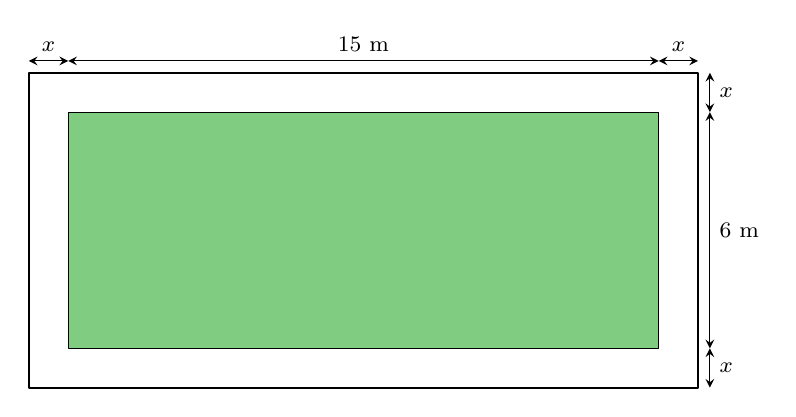
\begin{tikzpicture}[line join = round, line cap=round,>=stealth,font=\footnotesize,scale=0.5]
			\draw[thick] (0,0)--(0,8)--(17,8)--(17,0)--cycle;
			\draw[fill=green!60!black!50] (1,1)--(1,7)--(16,7)--(16,1)--cycle;
			\draw[<->] (0,8.3)--(1,8.3)node[midway,above]{$x$};
			\draw[<->] (1,8.3)--(16,8.3)node[midway,above]{$15$ m};
			\draw[<->] (16,8.3)--(17,8.3)node[midway,above]{$x$};
			\draw[<->] (17.3,0)--(17.3,1)node[midway,right]{$x$};
			\draw[<->] (17.3,1)--(17.3,7)node[midway,right]{$6$ m};
			\draw[<->] (17.3,7)--(17.3,8)node[midway,right]{$x$};
		\end{tikzpicture}
	\end{center}
	\begin{enumerate}
		\item Hãy viết biểu thức tính diện tích lối đi theo $x$.
		\item Hãy tính chiều rộng $x$ của lối đi, biết lối đi có diện tích là $100$ m$^2$.
	\end{enumerate}
	\loigiai
	{
		\begin{enumerate}
			\item Điều kiện: $x>0$.\\
			Diện tích nền đất hình chữ nhật là $(2x+15)\cdot (2x+6)=4x^2+42x+90$ (m$^2$).\\
			Diện tích sân cỏ hình chữ nhật là $15\cdot 6=90$ (m$^2$).\\
			Diện tích lối đi là $4x^2+42x+90-90=4x^2+42x$ (m$^2$).
			\item Vì lối đi có diện tích là $100$ m$^2$ do đó
			\begin{eqnarray*}
				4x^2+42x &=& 100\\
				4x^2+42x-100 &=& 0\\
				x = 2  &\textrm{ hoặc }& x=-\dfrac{25}{2}.
			\end{eqnarray*}
			Vì $x > 0$ nên $x = 2$.\\
			Vậy chiều rộng của lối đi là $2$ m.
		\end{enumerate}
	}
\end{bt} 

\begin{bt}%[9D4V2-5]%[GVSB: Nguyễn Văn Nghĩa-GVPB1:Hoàng Minh Nhân Mã-GVPB2: Phan Tấn Phú]
	Một khu vườn hình chữ nhật có chu vi $80$ m. Người ta để một lối đi xung quanh vườn rộng $2$ m. Phần đất còn lại dùng để trồng hoa có diện tích là $156$ m$^2$ (Hình bên dưới). Tính chiều rộng và chiều dài của khu vườn đó.
	\begin{center}
		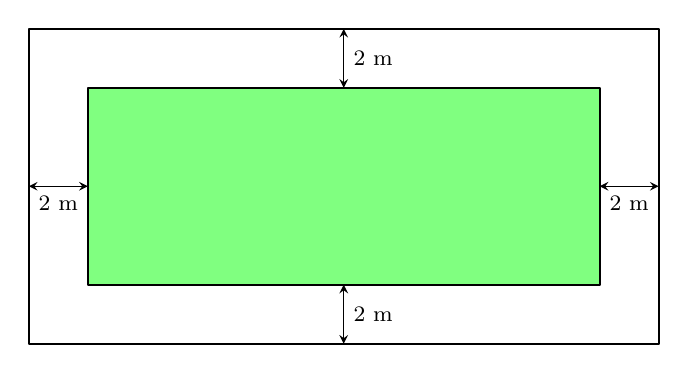
\begin{tikzpicture}[scale=1, font=\footnotesize, line join=round, line cap=round, >=stealth]
			\draw [thick] (0,0) rectangle (8,4);
			\fill [green!50] (0.75,0.75) rectangle (7.25,3.25);
			\draw [thick] (0.75,0.75) rectangle (7.25,3.25);
			\draw[<->](0,2)--node[midway,below]{$2$ m}(0.75,2);
			\draw[<->](7.25,2)--node[midway,below]{$2$ m}(8,2);		
			\draw[<->](4,3.25)--node[midway,right]{$2$ m}(4,4);		
			\draw[<->](4,0)--node[midway,right]{$2$ m}(4,.75);	
		\end{tikzpicture}
	\end{center}
	\loigiai{Nửa chu vi khu vườn hình chữ nhật là $80:2=40$ (m).\\
		Gọi $x$ (m) là chiều dài của khu vườn hình chữ nhật ($20<x<40$).\\
		Suy ra chiều rộng của khu vườn hình chữ nhật là $40-x$ (m).\\	
		Vì mỗi bên để $2$ (m) nên chiều dài của phần đất để trồng hoa chỉ còn $x-4$ (m) và chiều rộng là $40-x-4=36-x$ (m).\\
		Vì diện tích trồng hoa là $156$ m$^2$ nên ta có phương trình 
		\allowdisplaybreaks	 
		\begin{eqnarray*}
			(x-4)(36-x)&=&156\\
			x^2-40x+300&=&0\\
			x^2-10x-30x-300&=&0\\
			x(x-10)-30(x-10)&=&0\\
			(x-10)(x-30)&=&0\\	 
			x=10 &\text{hoặc}&x=30.	 
		\end{eqnarray*}
		Ta có $x=30$ thỏa mãn  điều kiện. \\	
		Vậy chiều dài của khu vườn là $30$ (m) và chiều rộng là $40-30=10$ (m).	
	}
\end{bt} 

\begin{bt}%[9D4V2-5]%[GVSB: Nguyễn Văn Nghĩa-GVPB1:Hoàng Minh Nhân Mã-GVPB2: Phan Tấn Phú]
	\immini{Ông Thành có một mảnh đất hình chữ nhật có chiều rộng là $8$ m và chiều dài là $20$ m. Nhà nước làm một con đường đi ngang qua mảnh đất của ông Thành và thu hồi một phần đất của ông Thành (phần hình tam giác). Phần đất không bị thu hồi có kích thước như hình vẽ bên (phần tô đậm).}
	{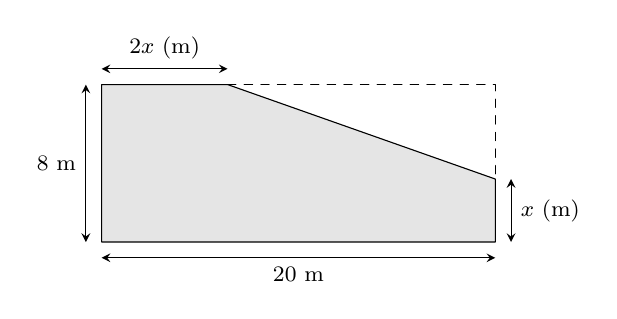
\begin{tikzpicture}[line join = round, line cap=round,>=stealth,font=\footnotesize,scale=1]
			\def\dai{5} \def\rong{2} \def\c{0.8} \def\d{0.2}
			\path 
			(0,0) coordinate (A)
			(90:\rong) coordinate (B)
			(\c*2,\rong) coordinate (C)
			(\dai,\c) coordinate (D)
			(0:\dai) coordinate (E)
			(\dai,\rong) coordinate (X)
			;
			\draw[fill=lightgray!40] (A)--(B)--(C)--(D)--(E)--cycle;
			\draw[dashed] (C) -- (X) --(D);
			\draw[<->] (A)++(180:\d)--++(90:\rong) node[midway,left]{$8$ m};
			\draw[<->] (B)++(90:\d)--++(0:\c*2) node[midway,above]{$2x$ (m)};
			\draw[<->] (E)++(0:\d)--++(90:\c) node[midway,right]{$x$ (m)};
			\draw[<->] (A)++(-90:\d)--++(0:\dai) node[midway,below]{$20$ m};
		\end{tikzpicture}	
	}
	\begin{enumerate}
		\item Viết biểu thức (thu gọn) $T$ biểu thị theo $x$ (với $0<x<8$) diện tích đất bị thu hồi của nhà ông Thành.
		\item Ông Thành được đền bù số tiền $455$ triệu đồng cho diện tích đất bị thu hồi. Tìm giá trị $x$ (m) biết giá đền bù đất bị thu hồi là $13$ triệu đồng/m$^2$.
	\end{enumerate}
	\loigiai
	{
		\begin{enumerate}
			\item Biểu thức $T$ biểu thị theo $x$ diện tích đất bị thu hồi của nhà ông Thành là
			$$T=\dfrac{1}{2}(20-2x)(8-x) = x^2-18x+80 \textrm{ (m$^2$) với $0<x<8$.}$$ 
			\item Vì ông Thành được đền bù số tiền $455$ triệu đồng cho diện tích đất bị thu hồi nên ta có phương trình
			\allowdisplaybreaks
			\begin{eqnarray*}
				\left( x^2-18x+80\right) \cdot13&=&455\\
				x^2-18x+80&=&35\\
				x^2-18x+45&=&0
			\end{eqnarray*}
			Giải phương trình trên, ta được $x=15$ (loại) hoặc $x=3$ (nhận).\\
			Vậy $x=3$ m.
		\end{enumerate}
	}
\end{bt}

\begin{bt}%[9D4V2-5]%[GVSB: Nguyễn Văn Nghĩa-GVPB1:Hoàng Minh Nhân Mã-GVPB2: Phan Tấn Phú]
	\immini{Một mảnh vườn hình vuông sau khi mở rộng mỗi cạnh $5$ m thì được một mảnh vườn hình vuông với cạnh là $x$ (m) như hình vẽ.
		\begin{enumerate}
			\item Viết biểu thức (dạng đa thức thu gọn) biểu thị diện tích mảnh vườn trước khi mở rộng.
			\item Biết rằng khi sau khi mở rộng diện tích mảnh vườn tăng lên $145$ m$^2$ so với diện tích ban đầu. Tìm giá trị của $x$?
		\end{enumerate}
	}{
		\begin{tikzpicture}[declare function={r=3;},scale=1,>=stealth, font=\footnotesize,line join=round,line cap=round]
			\path 
			% hình vuông lớn
			(0:0) coordinate (A)
			(0:r) coordinate (B)
			(90:r) coordinate (D)
			($(B)+(D)-(A)$) coordinate (C)
			%hình vuông nhỏ
			($(A)!0.5!(D)$) coordinate (E)
			($(A)!0.5!(B)$) coordinate (F)
			($(E)+(F)-(A)$) coordinate (G)
			;
			\draw[fill=gray!60] 
			(A)--(E)--(G)--(F)--cycle
			;
			\draw 
			(A)--(B)--(C)--(D)--cycle
			;
			\path
			(D)--(C) node[above,midway] {$x$}
			(B)--(C) node[midway, right] {$x$}
			;
			%
			\path 
			(D)++(180:7pt) coordinate (D1)
			(E)++(180:7pt) coordinate (E1)
			(B)++(-90:7pt) coordinate (B1)
			(F)++(-90:7pt) coordinate (F1)
			;
			\draw[|<->|]
			(D1)--(E1) node[midway,left] {$5$}
			;
			\draw[|<->|]
			(F1)--(B1) node[midway,below] {$5$}
			;
		\end{tikzpicture}
	}
	\loigiai{
		\begin{enumerate}
			\item Cạnh mảnh vườn hình vuông trước khi mở rộng là $x-5$ (m).\\
			Biểu thức biểu thị diện tích mảnh vườn hình vuông trước khi được mở rộng là
			$$(x-5)^2=x^2-10x+25.$$
			\item Do sau khi mở rộng diện tích mảnh vườn tăng lên $145$ m$^2$ so với diện tích ban đầu nên ta được phương trình
			\begin{eqnarray*}
				x^2-(x^2-10x+25)&=&145\\
				x^2-x^2+10x-25&=&145\\
				10x&=&170\\
				x&=&17.
			\end{eqnarray*}
			Vậy $x=17$ mét.
		\end{enumerate}
	}
\end{bt}
